\chapter{Opis projektnog zadatka}
		
		Ova web aplikacija omogućuje donatorima krvi da uz što manje muke nađu najbliže lokacije darivanja krvi te im daje mogućnost prisustvovanja u 				raznim akcijama organiziranih od Crvenog Križa ili drugih zavoda. Donor ima pristup svojoj povijesti darivanja što mu omogućava lako izdavanje 					potvrde od prošlih darivanje te datum isteka perioda čekanja ( od svakog darivanja krvi treba proći 4-6 mjeseci ovisno o spolu, radi tetovaža…). 					Svakim darivanjem krvi donor skuplja mogućnost za razne bonuse.
		
		Crvenom Križu i ostalim zavodima ova aplikacija omogućuje lakše organiziranje akcija u slučaju manjka krvi na nekoj lokaciji. Preko aplikacije 					dodjeljuju priznanja, izdavaju potvrde i davaju pozivnice. Također imaju evidenciju o svim darivateljima (ime, prezime, krvna grupa). Zadaća 					administratora je verificiranje podataka te davanje dopuštenja za darivanje.

		Ova aplikacija bi bila u interesu svih ljudi koji su zainteresirani za darivanje krvi, onih koji žele nešto o tome naučiti te onih koji ih organiziraju. Zbog 				lake uporabe lako povezuje donore s mjestima u krizi (bolnicama, organizacijama). Također omogućava povezanost između mjesta darivanja jer im 				daje uvit koliko koje krvi ima koja ustanova.

		Prilikom pokretanja stranice pojavljuje se karta Republike Hrvatske s označenim lokacijama (Zavod za transfuziju KBC Osijek, KBC Rijeka, KBC Split, OB 		Dubrovnik, OB Varaždin, OB Zadar i Hrvatski zavod za transfuzijsku medicinu Zagreb) te prozor s akcijama Crvenog Križa u Hrvatskoj. Klikom na 					lokacije pojavi se prozor u kojem se nalaze akcije za tu lokaciju, postotci zaliha krvi te gumb za prijavu za donaciju. Neregistriranog korisnika stranica 				vodi na registraciju, a korisniku prikazuje registracijski obrazac za donaciju. 
		Neregistrirani korisnik se može prijaviti u aplikaciju kao:

		\begin{packed_item}
			\item donor –  pojavljuju mu se skočni prozorčići s pozivima Crvenog Križa na donacije i akcije, omogućena mu je kontrola osobnih 							podataka, prijava na donacije i akcije, statistika vlastitog doniranja, ispis potvrda i zahtjev za nagradama od Crvenog Križa i drugih zavoda te 					brisanje korisničkog računa
				\begin{packed_item}
					\item potrebne informacije za registraciju
				\end{packed_item}
			\item Crveni Križ – omogućeno mu je objavljivanje akcija, izdavanje potvrda, dodjela priznanja te verificiranje podataka
				\begin{packed_item}
					\item potrebne informacije za registraciju
				\end{packed_item}
			\item zavodi – omogućen uvid u popis donora, brisanje donorskih korisničkih računa i izdavanje akcija
				\begin{packed_item}
					\item potrebne informacije za registraciju
				\end{packed_item}
		\end{packed_item}
		
		Administratori su osobe zaslužne za održavanje aplikacije te se neregistriranom korisniku ne daje pristup prijave kao administrator. 

		Sustav treba podržavati rad više korisnika u stvarnom vremenu.

		Slične web aplikacije:
		\begin{packed_item}
			\item  „GiveBlood“ ( https://www.redcross.org/give-blood.html ):
			Na početnoj web stranici nalaze se obavijesti vezane za različite krvne grupe, krvnu plazmu te različite zanimljivosti vezane uz temu. U alatnoj 					traci nalaze se često pitana pitanja koja su grupirana po temama ( „sve o plazmi“, „zašto dati krv“, „tko može dati krv“,  „proces donacije“). Tu se 			također nalazi tražilica koja traži najbliže lokacije u Engleskoj gdje se može donirati te link s aktualnim zdravstvenim vijestima. Korisnici imaju 					mogućnost prijave i rezervacije termina za donaciju.
			\begin{figure}[H]
				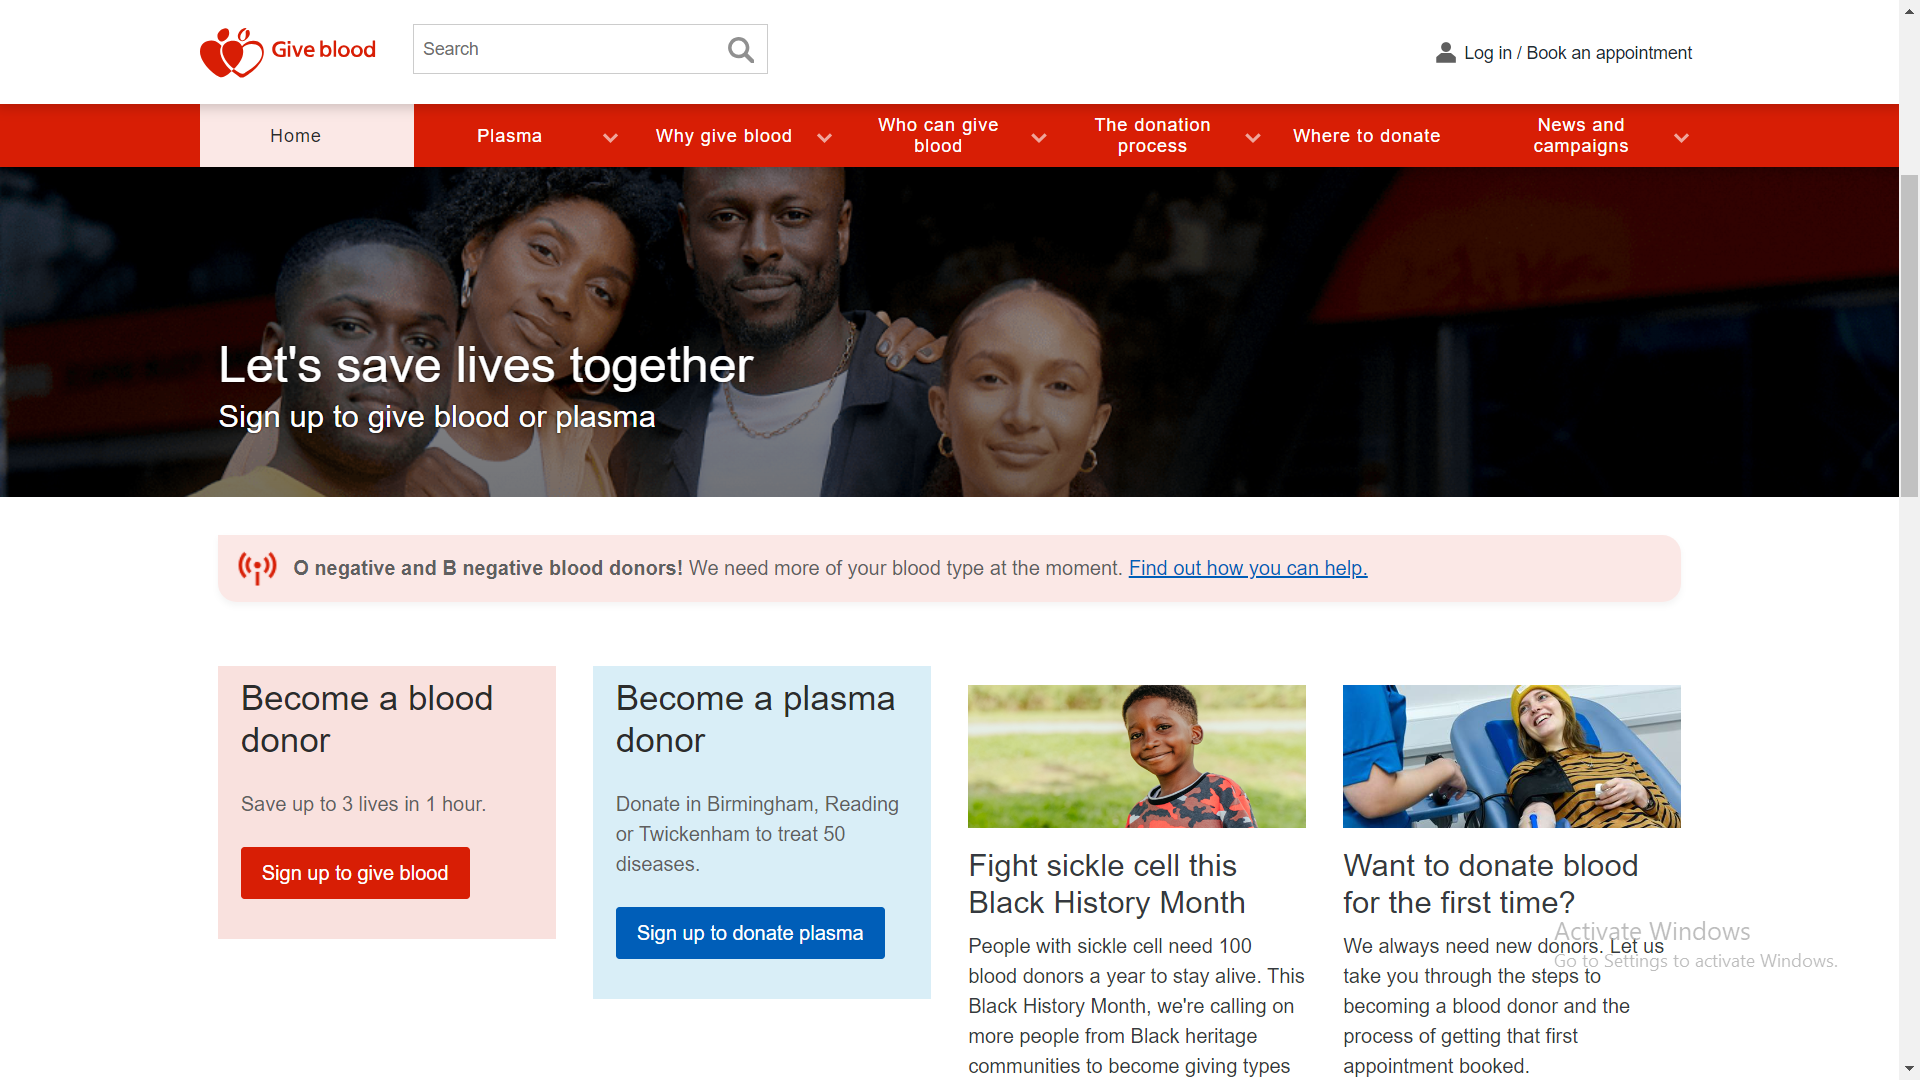
\includegraphics[scale=0.23]{slike/giveblood.PNG} 
				\centering
				\caption{Prikaz glavne stranice GiveBlood-a}
				\label{fig:promjene}
			\end{figure}
			\item „friends2support“ ( https://www.friends2support.org/index.aspx ):
			Web stranica traži davatelje krvi diljem svijeta. Korisnik može unijeti krvnu grupu, državu, županiju, okrug i grad te aplikacija na temelju toga 					traži donatore. Korisnik ima mogućnost registracije. Na stranici se također nalaze razne vijesti, videa i slike o darivanju krvi.
			\begin{figure}[H]
				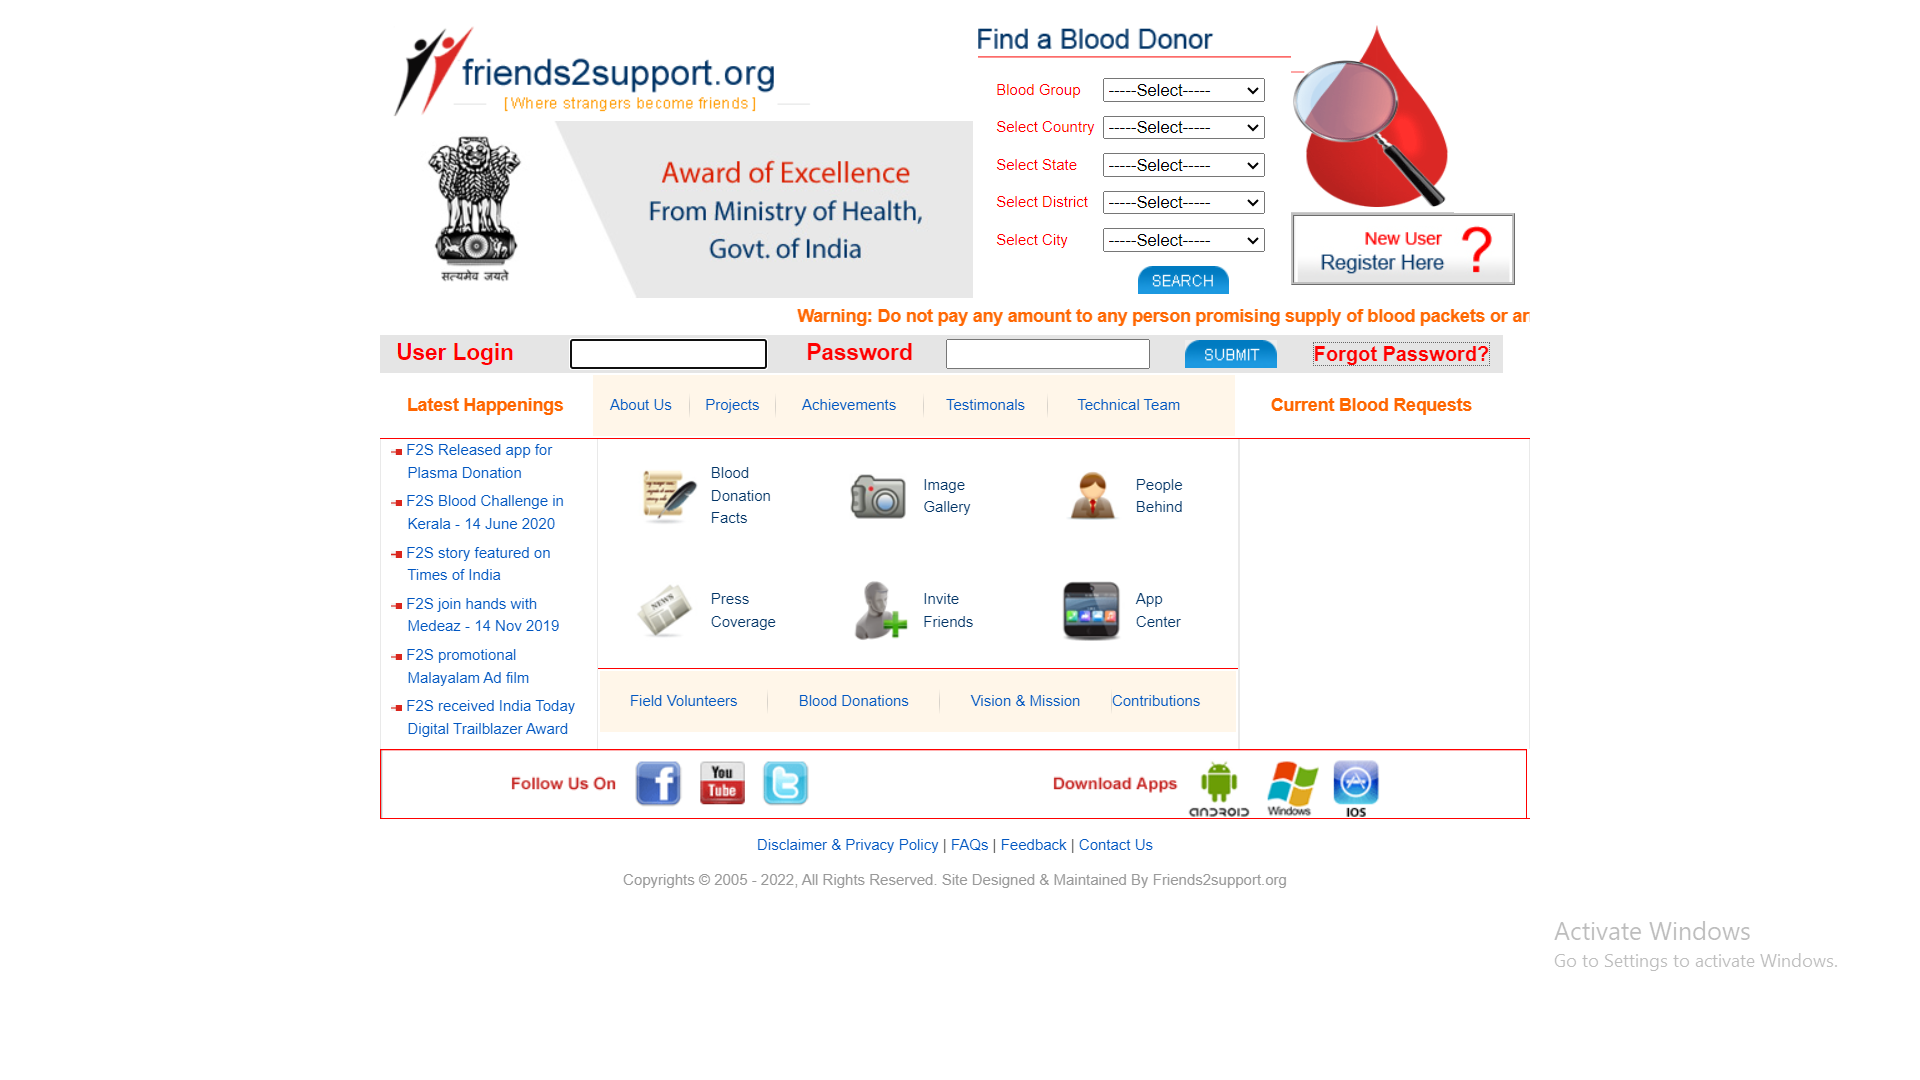
\includegraphics[scale=0.23]{slike/friends2support.PNG} 
				\centering
				\caption{Prikaz glavne stranice friends2support-a}
				\label{fig:promjene}
			\end{figure}
			\item  „vitalant“ ( https://vitalant.org/ ):
			Na početnoj stanici nalaze se elementi preko kojih korisnik  može zakazati termin donacije, naučiti o donaciji te saznati je li poželjni donor. 						Također iskaču aktualne vijesti ili nagradne igre. Na alatnoj traci nalaze se razna pitanja i članci grupirani po temama (o donaciji, o krvi,  o 						poželjnosti, o volonterima i o bolnicama).
			\begin{figure}[H]
				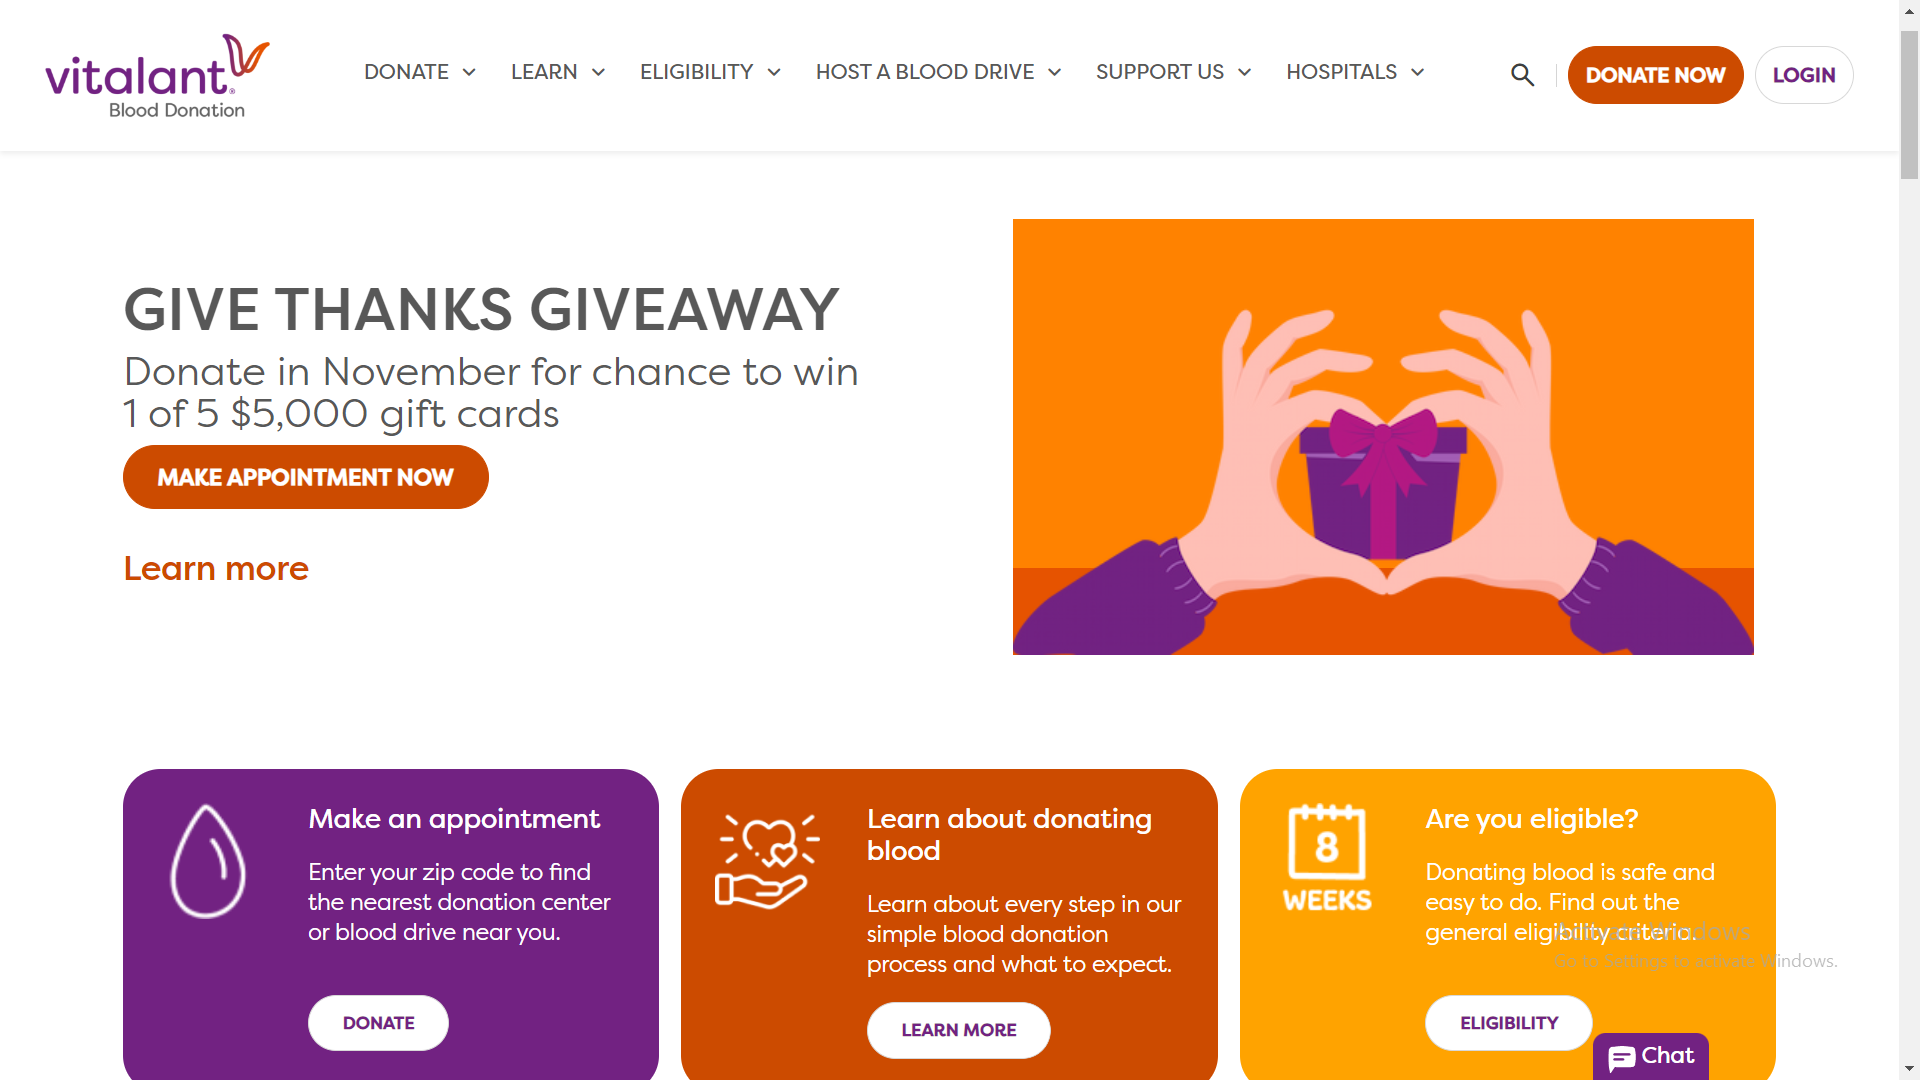
\includegraphics[scale=0.23]{slike/vitalant.PNG} 
				\centering
				\caption{Prikaz glavne stranice vitalant-a}
				\label{fig:promjene}
			\end{figure}
		\end{packed_item}

		\eject
		
		\section{Primjeri u \LaTeX u}
		
		\textit{Ovo potpoglavlje izbrisati.}\\

		U nastavku se nalaze različiti primjeri kako koristiti osnovne funkcionalnosti \LaTeX a koje su potrebne za izradu dokumentacije. Za dodatnu pomoć obratiti se asistentu na projektu ili potražiti upute na sljedećim web sjedištima:
		\begin{itemize}
			\item Upute za izradu diplomskog rada u \LaTeX u - \url{https://www.fer.unizg.hr/_download/repository/LaTeX-upute.pdf}
			\item \LaTeX\ projekt - \url{https://www.latex-project.org/help/}
			\item StackExchange za Tex - \url{https://tex.stackexchange.com/}\\
		
		\end{itemize} 	


		
		\noindent \underbar{podcrtani tekst}, \textbf{podebljani tekst}, 	\textit{nagnuti tekst}\\
		\noindent \normalsize primjer \large primjer \Large primjer \LARGE {primjer} \huge {primjer} \Huge primjer \normalsize
				
		\begin{packed_item}
			
			\item  primjer
			\item  primjer
			\item  primjer
			\item[] \begin{packed_enum}
				\item primjer
				\item[] \begin{packed_enum}
					\item[1.a] primjer
					\item[b] primjer
				\end{packed_enum}
				\item primjer
			\end{packed_enum}
			
		\end{packed_item}
		
		\noindent primjer url-a: \url{https://www.fer.unizg.hr/predmet/proinz/projekt}
		
		\noindent posebni znakovi: \# \$ \% \& \{ \} \_ 
		$|$ $<$ $>$ 
		\^{} 
		\~{} 
		$\backslash$ 
		
		
		\begin{longtblr}[
			label=none,
			entry=none
			]{
				width = \textwidth,
				colspec={|X[8,l]|X[8, l]|X[16, l]|}, 
				rowhead = 1,
			} %definicija širine tablice, širine stupaca, poravnanje i broja redaka naslova tablice
			\hline \SetCell[c=3]{c}{\textbf{naslov unutar tablice}}	 \\ \hline[3pt]
			\SetCell{LightGreen}IDKorisnik & INT	&  	Lorem ipsum dolor sit amet, consectetur adipiscing elit, sed do eiusmod  	\\ \hline
			korisnickoIme	& VARCHAR &   	\\ \hline 
			email & VARCHAR &   \\ \hline 
			ime & VARCHAR	&  		\\ \hline 
			\SetCell{LightBlue} primjer	& VARCHAR &   	\\ \hline 
		\end{longtblr}
		

		\begin{longtblr}[
				caption = {Naslov s referencom izvan tablice},
				entry = {Short Caption},
			]{
				width = \textwidth, 
				colspec = {|X[8,l]|X[8,l]|X[16,l]|}, 
				rowhead = 1,
			}
			\hline
			\SetCell{LightGreen}IDKorisnik & INT	&  	Lorem ipsum dolor sit amet, consectetur adipiscing elit, sed do eiusmod  	\\ \hline
			korisnickoIme	& VARCHAR &   	\\ \hline 
			email & VARCHAR &   \\ \hline 
			ime & VARCHAR	&  		\\ \hline 
			\SetCell{LightBlue} primjer	& VARCHAR &   	\\ \hline 
		\end{longtblr}
	


		
		
		%unos slike
		\begin{figure}[H]
			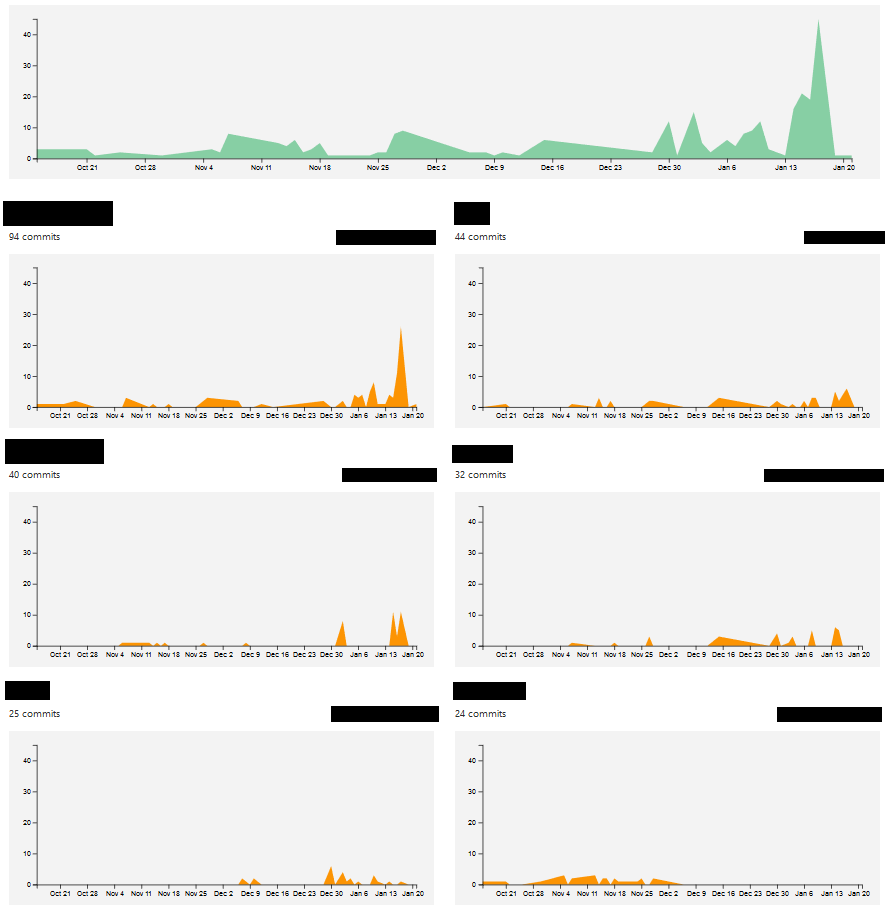
\includegraphics[scale=0.4]{slike/aktivnost.PNG} %veličina slike u odnosu na originalnu datoteku i pozicija slike
			\centering
			\caption{Primjer slike s potpisom}
			\label{fig:promjene}
		\end{figure}
		
		\begin{figure}[H]
			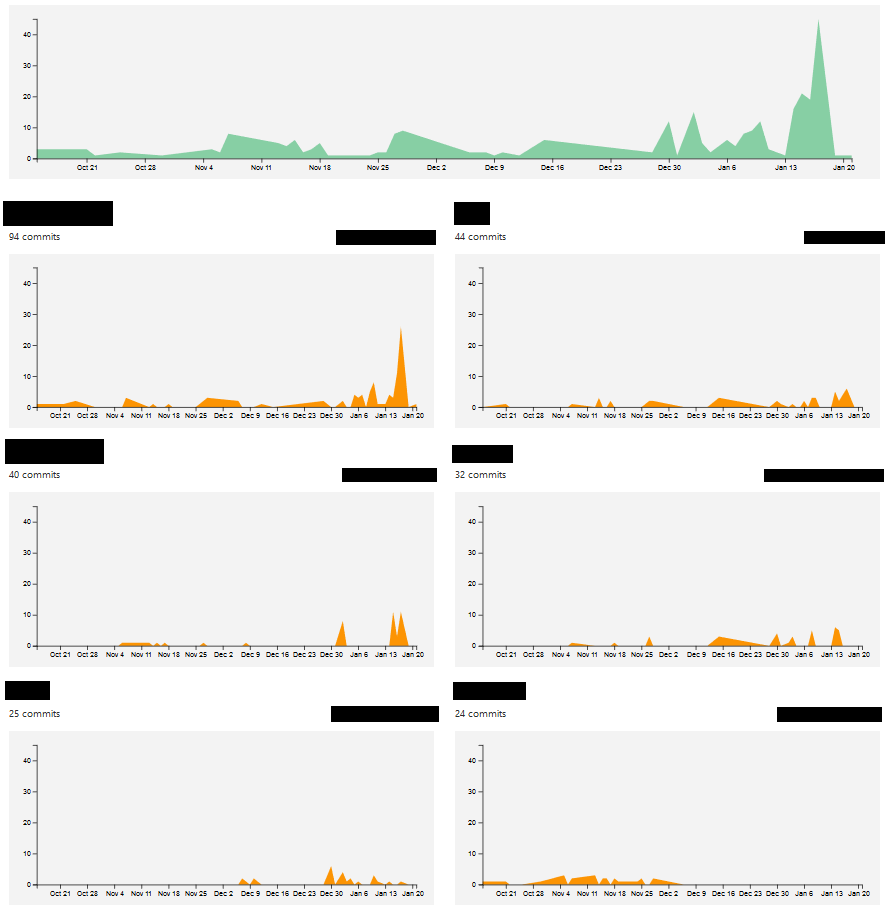
\includegraphics[width=\textwidth]{slike/aktivnost.PNG} %veličina u odnosu na širinu linije
			\caption{Primjer slike s potpisom 2}
			\label{fig:promjene2} %label mora biti drugaciji za svaku sliku
		\end{figure}
		
		Referenciranje slike \ref{fig:promjene2} u tekstu.
		
		\eject
		
	